\documentclass[../main.tex]{subfiles}
\begin{document}
%=========================================================
% TĐ_GiaoAn_IQA_HK1_Tuan15_Thoigian
% Giáo án Toán tư duy cấp độ A - Chủ đề THỜI GIAN (Buổi 1, Buổi 2)
% Soạn theo mẫu giáo án (\hktuan, \subsection, hd, vd, luuy)
% Hình đặt trong thư mục Hinh_Tuan15/ (các hình của giáo án có tiền tố ga_)
\graphicspath{{Hinh_Tuan15/}{Data_GiaoAn_HK0/Hinh_Tuan15/}}%biên dịch riêng file này hoặc từ main.tex đều được
%=========================================================

%---------- Lệnh dùng riêng cho giáo án ----------
% Chèn hình (mặc định rộng 12cm, căn giữa)
\providecommand{\TThinh}[2][12cm]{\begin{center}\includegraphics[width=#1,height=0.9\textheight,keepaspectratio]{#2}\end{center}}
% Mục nhỏ a), b), c) trong một hoạt động
\providecommand{\GAmucnho}[1]{\par\addvspace{4pt}\noindent{\color{mauchinh}\bfseries #1}\par\nopagebreak\addvspace{2pt}}
% Đồng hồ trống có ghi số phút 0, 5, ..., 55 xung quanh (hình vẽ trên bảng)
\providecommand{\GAdonghophut}{%
  \begin{center}
    \begin{tikzpicture}
      \node at (0,0) {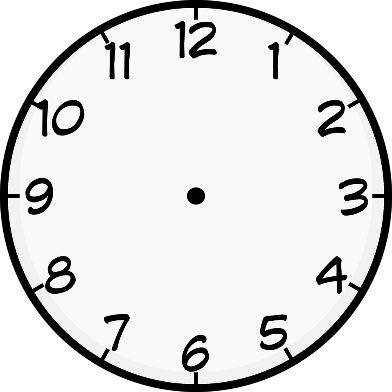
\includegraphics[width=4.5cm]{ga_image8.png}};
      \foreach \k in {0,...,11}{%
        \node[font=\small\bfseries,text=mauchinh] at ({90-30*\k}:2.95cm) {\number\numexpr5*\k\relax};}
    \end{tikzpicture}
  \end{center}}

%%%%%%%%%%%%%%%%%%%%%%%%%%%%%%%%%%%%%%%%%%%%%%%%%%%%%%%%%%
%                       BUỔI 1
%%%%%%%%%%%%%%%%%%%%%%%%%%%%%%%%%%%%%%%%%%%%%%%%%%%%%%%%%%
%\setcounter{section}{3} % không chỉnh sửa
\hktuan{1}{15}
%\textbf{Người soạn: }
\begin{center}
        {\color{mauchinh!120}\bfseries\Large THỜI GIAN (BUỔI 1)}
\end{center}

\subsection{MỤC TIÊU CẦN ĐẠT}
\begin{itemize}
    \item HS phân biệt được các loại kim: kim giờ, kim phút, kim giây.
    \item HS biết xem đồng hồ: biết cách đọc giờ đúng, giờ 24, giờ rưỡi và giờ lẻ (giờ có phút, đối với HS nhanh).
    \item HS biết cách vẽ giờ đúng.
\end{itemize}

\subsection{TIẾN TRÌNH DẠY HỌC}
\textbf{Đồ dùng dạy học:} giáo án, PBT, bút, khăn ẩm, laptop, con dấu, đồng hồ.

%---------------------------------------------------------
\subsubsection{ỔN ĐỊNH LỚP. SỬA BÀI TẬP VỀ NHÀ}
\begin{hd}
    \begin{itemize}
        \item Thời gian: 10 phút
        \item Ổn định lớp, sửa bài tập về nhà.
    \end{itemize}
\end{hd}

%---------------------------------------------------------
\subsubsection{XEM ĐỒNG HỒ}
\begin{hd}
    \begin{itemize}
        \item Thời gian: 50 phút
        \item HS phân biệt kim giờ, kim phút; biết vị trí các số trên mặt đồng hồ.
        \item HS đọc được giờ đúng, giờ 24 và giờ lẻ (HS nhanh).
    \end{itemize}
\end{hd}
\begin{itemize}
    \item GV vấn đáp HS một số câu hỏi:
    \begin{itemize}
        \item Chúng ta xem giờ bằng gì?
        \item Đồng hồ thường có hình dạng gì?
    \end{itemize}
    \item Giới thiệu với HS một số loại đồng hồ: đồng hồ đeo tay, đồng hồ báo thức, đồng hồ treo tường,\dots
\end{itemize}
\begin{center}
    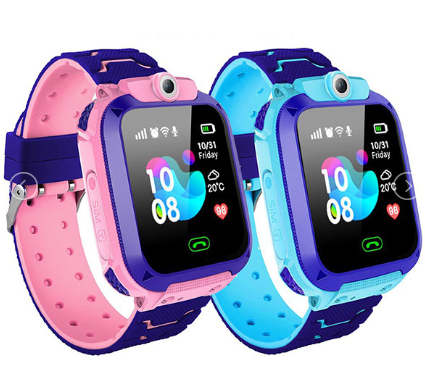
\includegraphics[width=4cm]{ga_image1.png}\hspace{1cm}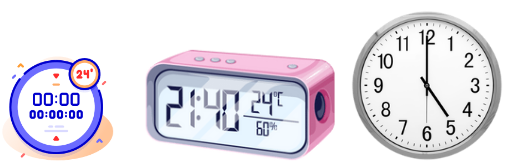
\includegraphics[width=7.4cm]{ga_image2.png}
\end{center}

\GAmucnho{Trò chơi “Hai chiếc kim”}
\begin{itemize}
    \item GV chuẩn bị: đồng hồ treo tường 2 kim (hoặc đồng hồ mô hình), hình “Hai chiếc kim” bên dưới.
    \item Cách chơi: GV kể: “Hai bạn kim cùng xuất phát ở số 12, thi chạy một vòng quanh đồng hồ. Con đoán xem ai về đích trước?”. HS đoán, giơ tay bình chọn. GV xoay kim phút một vòng, kim giờ nhích sang số kế tiếp để cả lớp kiểm chứng.
    \item GV vấn đáp: Nếu kim phút (kim dài) quay một vòng thì kim giờ (kim ngắn) di chuyển như thế nào?
    \item GV hướng dẫn và làm mẫu cho HS theo từng cấp độ.
\end{itemize}
\TThinh[13.2cm]{ga_image3.png}
\begin{luuy}
    \begin{itemize}
        \item Kim phút chạy nhanh hơn kim giờ. Kim ngắn chỉ giờ, kim dài chỉ phút.
        \item Kim phút quay một vòng thì kim giờ di chuyển từ số này đến số kế tiếp.
    \end{itemize}
\end{luuy}

\GAmucnho{Trò chơi “Điền số thần tốc”}
\begin{itemize}
    \item Chia lớp 2 đội. GV vẽ đồng hồ lên bảng cho HS quan sát, chú ý vị trí của các số 12, 3, 6, 9. GV xóa các số, chỉ để lại các số 12, 3, 6, 9 và yêu cầu HS điền các số ở giữa.
    \item Mỗi lượt, một bạn của mỗi đội chạy lên điền nhanh một số còn thiếu trên đồng hồ vẽ ở bảng (GV đã xóa dần). Đội điền đúng và nhanh hơn được 1 sao. Tiếp tục như vậy đến khi HS nắm được vị trí các số trên đồng hồ.
\end{itemize}
\begin{luuy}
    Mẹo nhớ: \textit{“12 ở đỉnh đầu, 6 ở dưới chân, 3 bên phải, 9 bên trái.”}
\end{luuy}
\TThinh[9.7cm]{ga_image4.png}

\GAmucnho{a) Giờ đúng}
\begin{itemize}
    \item Giữ kim phút ở số 12, di chuyển kim giờ qua các số 1, 2, 3, \dots hướng dẫn HS đây là giờ đúng và đọc là 1 giờ, 2 giờ, 3 giờ, \dots
    \item GV xoay kim, lần lượt gọi từng HS đọc giờ, thực hiện nhiều lần để HS nhớ.
    \item Giới thiệu cho HS cách ghi giờ bằng dấu hai chấm: 5:00, 9:00, \dots
    \item GV chia lớp thành nhóm 2 -- 3 HS thi đua xoay đồng hồ theo yêu cầu của GV để lấy điểm cộng.
\end{itemize}
\begin{luuy}
    Một số trường hợp đặc biệt: 12 giờ (kim giờ và kim phút trùng nhau), 6 giờ (kim phút và kim giờ thẳng hàng).
\end{luuy}
\begin{vd}
    Kim phút chỉ số 12, kim giờ chỉ số 5 $\Rightarrow$ đồng hồ chỉ \textbf{5 giờ}, viết là \textbf{5:00}.
\end{vd}
\textbf{Bài tập áp dụng:} Bài 1, 2, 3 Phiếu bài tập.

\GAmucnho{b) Đọc giờ 24}
\begin{itemize}
    \item Giới thiệu cho HS biết 1 ngày có 24 giờ $\Rightarrow$ kim giờ sẽ chạy 2 vòng đồng hồ.
    \item Giới thiệu với HS các buổi trong ngày (sáng, trưa, chiều, tối). GV dựa vào việc quan sát không gian xung quanh: buổi sáng (trưa, chiều, tối) sẽ như thế nào?
    \item GV cho HS chơi \textbf{“Một ngày của em”} (dán thẻ lên trục thời gian):
    \begin{itemize}
        \item Chuẩn bị: 4 -- 6 thẻ tranh hoạt động (thức dậy, đi học, ăn trưa, tan học, ăn tối, đi ngủ); vẽ trục thời gian lên bảng như hình dưới.
        \item Cách chơi: mỗi nhóm nhận 1 thẻ, cử đại diện dán thẻ vào đúng buổi (sáng -- chiều -- tối).
    \end{itemize}
\end{itemize}
\TThinh[16.4cm]{ga_image5.png}
\begin{itemize}
    \item GV hướng dẫn: qua 12 giờ trưa, kim phút chỉ số 12, kim giờ chỉ số 1 đọc là 1 giờ chiều hoặc là 13 giờ; tương tự với các giờ tiếp theo.
    \item GV vừa hướng dẫn vừa điền vào bảng và vấn đáp để HS ghi nhớ.
\end{itemize}

% Bảng SÁNG - CHIỀU - TỐI (chứa 2 bảng con)
\begin{center}
    \renewcommand{\arraystretch}{1.3}
    \setlength{\tabcolsep}{3pt}
    \begin{tabular}{|p{1.7cm}|p{8cm}|p{6.7cm}|}
        \hline
        \centering\textbf{SÁNG} & \centering\textbf{CHIỀU} & \centering\arraybackslash\textbf{TỐI} \\ \hline
        0 giờ đến 12 giờ (1 vòng đồng hồ)
        &
        {\scriptsize\setlength{\tabcolsep}{1.5pt}\renewcommand{\arraystretch}{1.2}%
        \begin{tabular}{|*{6}{>{\centering\arraybackslash}p{1.2cm}|}}
            \hline
            1 giờ chiều & 2 giờ chiều & 3 giờ chiều & 4 giờ chiều & 5 giờ chiều & 6 giờ chiều \\ \hline
            13 giờ & 14 giờ & 15 giờ & 16 giờ & 17 giờ & 18 giờ \\ \hline
        \end{tabular}}
        &
        {\scriptsize\setlength{\tabcolsep}{1.5pt}\renewcommand{\arraystretch}{1.2}%
        \begin{tabular}{|*{5}{>{\centering\arraybackslash}p{1.2cm}|}}
            \hline
            7 giờ tối & 8 giờ tối & 9 giờ tối & 10 giờ tối & 11 giờ tối \\ \hline
            19 giờ & 20 giờ & 21 giờ & 22 giờ & 23 giờ \\ \hline
        \end{tabular}} \\ \hline
    \end{tabular}
\end{center}

\begin{vd}
    GV vấn đáp HS, điền vào bảng:
    \begin{multicols}{2}
        \begin{itemize}
            \item 1 giờ chiều ứng với mấy giờ?
            \item 14 giờ ứng với mấy giờ chiều?
            \item 3 giờ chiều ứng với mấy giờ?
            \item Con đi học về lúc 17 giờ tức là mấy giờ chiều?
        \end{itemize}
    \end{multicols}
    \begin{center}
        \renewcommand{\arraystretch}{1.5}
        \begin{tabular}{|>{\centering\arraybackslash}p{4.5cm}|>{\centering\arraybackslash}p{4.5cm}|}
            \hline
            1 giờ chiều & ? \\ \hline
            ? & 14 giờ \\ \hline
            3 giờ chiều & ? \\ \hline
        \end{tabular}
    \end{center}
\end{vd}
\begin{itemize}
    \item GV vấn đáp HS tới khi HS đổi giờ được.
    \item \textbf{Bài tập áp dụng:} Bài 5 Phiếu bài tập.
    \item GV cho HS tập vẽ đồng hồ đúng và làm Bài 6 trong PBT.
\end{itemize}

\begin{center}
    {\color{mauchinh}\bfseries PHIẾU BÀI TẬP -- THỜI GIAN}
\end{center}
\TThinh[13cm]{ga_image6.png}
\TThinh[13.3cm]{ga_image7.png}

\GAmucnho{c) Giờ lẻ (giờ có phút) -- Đối với HS nhanh}
\begin{itemize}
    \item GV ôn lại đếm cách 5.
    \item GV cho HS chơi thi đua: các bạn đếm lần lượt 5, 10, 15, \dots, 55 sau đó quay lại; bạn nào đếm sai sẽ lên hát, múa,\dots Bạn nào sai ít nhất sẽ được cộng 3+, ít thứ hai được 2+, \dots
    \item GV quay lại bài học, di chuyển kim phút đến các vị trí 1, 2, \dots Giới thiệu cho HS mỗi vị trí ứng với số phút 5, 10, \dots
    \item GV vẽ đồng hồ và vị trí phút tương ứng để HS ghi nhớ. Chú ý cho HS các mốc đặc biệt cần nhớ để dễ đếm: 15, 30, 45 phút.
\end{itemize}
\GAdonghophut
\TThinh[7.1cm]{ga_image9.png}
\begin{itemize}
    \item GV di chuyển kim phút 1 vòng cho HS đọc phút và yêu cầu HS chú ý thêm về vị trí của kim giờ: khi kim phút quay thì kim giờ cũng quay theo.
    \item GV kết hợp với kim giờ để HS đọc giờ có phút.
    \item Đầu tiên di chuyển kim phút đến số 6 (30 phút). Yêu cầu HS đọc phút và quan sát vị trí của kim giờ lần nữa (nằm giữa số 2 và 3); tiếp tục quay kim phút sẽ thấy kim giờ từ từ di chuyển lại gần số 3.
    \item GV xoay kim phút trên đồng hồ rồi dừng tại một vài vị trí (20 phút, 35 phút,\dots), cả lớp viết số phút lên bảng con. GV vấn đáp, yêu cầu HS đọc giờ và phút đến khi cả lớp thành thạo.
    \item GV hướng dẫn HS đổi giờ lẻ theo cách đọc giờ 24 tương tự giờ đúng.
\end{itemize}
\begin{luuy}
    Khi \textbf{\textit{kim giờ chưa đến số 3}} thì đọc là \textbf{\textit{2 giờ \dots\ phút}}. Di chuyển đồng hồ bất kì và gọi HS đọc nhiều lần cho đến khi lớp đọc ổn.
\end{luuy}
\begin{vd}
    3 giờ 15 phút chiều tức là 15 giờ 15 phút; 18 giờ 30 phút tức là 6 giờ 30 phút tối.
\end{vd}
\begin{vd}
    GV vấn đáp HS:
    \begin{itemize}
        \item 1 giờ 45 phút chiều ứng với mấy giờ?
        \item 14 giờ 30 phút ứng với mấy giờ chiều?
        \item 7 giờ 20 phút tối ứng với mấy giờ?
        \item Con đi học Titan lúc 17 giờ 30 phút tức là mấy giờ chiều?
    \end{itemize}
\end{vd}

\GAmucnho{Trò chơi “Rung chuông vàng” (10 phút)}
\begin{itemize}
    \item Cách chơi: mỗi HS một bảng con. GV đọc câu hỏi, HS viết đáp án và giơ bảng khi nghe hiệu lệnh. Bạn nào sai ngồi xuống, bạn nào còn đứng đến cuối cùng được rung chuông vàng và nhận 3 sao cho nhóm. (Lớp từ 10 -- 20 HS có thể chơi theo nhóm: mỗi nhóm một bảng.)
    \item Câu hỏi gợi ý:
    \begin{itemize}
        \item 7 giờ tối là mấy giờ? $\rightarrow$ 19 giờ.
        \item Lúc 12 giờ, hai kim đồng hồ như thế nào? $\rightarrow$ Trùng nhau.
        \item Lúc 6 giờ, hai kim như thế nào? $\rightarrow$ Thẳng hàng.
        \item 20 giờ là mấy giờ tối? $\rightarrow$ 8 giờ tối.
        \item (HS nhanh) Kim phút chỉ số 6 là bao nhiêu phút? $\rightarrow$ 30 phút.
        \item (HS nhanh) 3 giờ 15 phút chiều đọc theo giờ 24 là? $\rightarrow$ 15 giờ 15 phút.
    \end{itemize}
\end{itemize}
\textbf{Bài tập áp dụng:} Bài 7 Phiếu bài tập.

%---------------------------------------------------------
\subsubsection{LUYỆN TẬP}
\begin{hd}
    \begin{itemize}
        \item Thời gian: 30 phút
        \item Củng cố kiến thức qua Phiếu bài tập.
    \end{itemize}
\end{hd}
\begin{itemize}
    \item GV cho HS làm bài trong PBT để củng cố kiến thức.
\end{itemize}

%---------------------------------------------------------
\subsubsection{BÀI TẬP VỀ NHÀ}
\begin{hd}
    \begin{itemize}
        \item Thời gian: 5 phút
    \end{itemize}
\end{hd}
\begin{itemize}
    \item GV giao BTVN tuỳ vào tình hình lớp.
\end{itemize}

%%%%%%%%%%%%%%%%%%%%%%%%%%%%%%%%%%%%%%%%%%%%%%%%%%%%%%%%%%
%                       BUỔI 2
%%%%%%%%%%%%%%%%%%%%%%%%%%%%%%%%%%%%%%%%%%%%%%%%%%%%%%%%%%
\newpage
\setcounter{subsection}{0}
\begin{center}
        {\color{mauchinh!120}\bfseries\Large THỜI GIAN (BUỔI 2)}
\end{center}

\subsection{MỤC TIÊU CẦN ĐẠT}
\begin{itemize}
    \item HS thành thạo đọc giờ đúng, biết vẽ kim đồng hồ tương ứng với giờ đúng.
    \item HS ước lượng được mốc thời gian thực hiện các hoạt động.
    \item HS ước lượng được khoảng thời gian thực hiện một hoạt động.
    \item HS tính được khoảng thời gian thực hiện một hoạt động theo yêu cầu.
\end{itemize}

\subsection{TIẾN TRÌNH DẠY HỌC}
\textbf{Đồ dùng dạy học:} giáo án, PBT, bút, khăn ẩm, laptop, con dấu, đồng hồ.

%---------------------------------------------------------
\subsubsection{ỔN ĐỊNH LỚP. SỬA BÀI TẬP VỀ NHÀ}
\begin{hd}
    \begin{itemize}
        \item Thời gian: 10 phút
        \item Ôn lại cách đọc giờ.
    \end{itemize}
\end{hd}
\begin{itemize}
    \item GV sửa bài tập về nhà cho HS, ôn lại cách đọc giờ và cho HS làm PBT buổi 2.
\end{itemize}

%---------------------------------------------------------
\subsubsection{ÔN TẬP XEM ĐỒNG HỒ, VẼ KIM ĐỒNG HỒ}
\begin{hd}
    \begin{itemize}
        \item Thời gian: 20 phút
        \item HS đọc giờ và vẽ kim đồng hồ với thời gian tương ứng.
    \end{itemize}
\end{hd}
\begin{itemize}
    \item GV cho HS ôn tập bằng cách chiếu hình 4 đồng hồ bên dưới. Mỗi đồng hồ có một bạn nhỏ “phát biểu” giờ. \textbf{Bạn nào đúng, bạn nào sai?} Gọi HS trả lời, giải thích và sửa lại đáp án cho đúng.
\end{itemize}
\TThinh[14.8cm]{ga_image10.png}
\begin{itemize}
    \item Gọi HS lên bảng vẽ kim đồng hồ.
    \item \textbf{Bài tập áp dụng:} Bài 1, 2 Phiếu bài tập.
\end{itemize}

%---------------------------------------------------------
\subsubsection{LẬP THỜI GIAN BIỂU. ƯỚC LƯỢNG KHOẢNG THỜI GIAN}
\begin{hd}
    \begin{itemize}
        \item Thời gian: 15 phút
        \item HS ước lượng mốc thời gian và khoảng thời gian của các hoạt động.
    \end{itemize}
\end{hd}
\GAmucnho{Lập thời gian biểu}
\begin{itemize}
    \item GV chuẩn bị các thẻ hoạt động và các thẻ ghi thời gian để phát cho HS.
    \item GV chia lớp thành nhóm 2 -- 3 HS để thi đua lấy điểm cộng.
    \item GV yêu cầu HS dán các thẻ thời gian phù hợp với các hoạt động: đi học, ăn cơm trưa, đi tắm, học bài, xem ti vi, đi ngủ,\dots
    \item Nhóm nào dán nhanh nhất sẽ được điểm cộng.
\end{itemize}
\GAmucnho{Ước lượng khoảng thời gian}
\begin{itemize}
    \item GV sử dụng đồng hồ bấm giờ cho HS ước lượng 10 giây, 1 phút, 5 phút,\dots
    \item Thời gian học của lớp mình là 1 giờ 30 phút, để HS ban đầu biết được 1 giây, 1 phút, 1 giờ là tầm bao nhiêu.
\end{itemize}
\textbf{Bài tập áp dụng:} Bài 4, 5 Phiếu bài tập.

%---------------------------------------------------------
\subsubsection{LUYỆN TẬP}
\begin{hd}
    \begin{itemize}
        \item Thời gian: 25 phút
    \end{itemize}
\end{hd}
\begin{itemize}
    \item GV cho HS làm bài trong PBT.
\end{itemize}

%---------------------------------------------------------
\subsubsection{TÍNH KHOẢNG THỜI GIAN}
\begin{hd}
    \begin{itemize}
        \item Thời gian: 10 phút (tùy vào tình hình mỗi lớp)
        \item HS tính được khoảng thời gian thực hiện một hoạt động.
    \end{itemize}
\end{hd}
\begin{itemize}
    \item GV cho một ví dụ đơn giản để HS làm quen với cách tính thời gian. Vấn đáp HS, bạn nào trả lời đúng được 1 điểm thưởng.
\end{itemize}
\TThinh[11.6cm]{ga_image13.png}
\begin{vd}
    \textbf{(Tiệc của Tom)} Buổi tiệc sinh nhật của bạn Tom bắt đầu lúc 16:00 và kết thúc lúc 18:30. Hỏi buổi tiệc sinh nhật của Tom kéo dài trong bao lâu?

    \textit{Hướng dẫn:} 16:00 $\rightarrow$ 17:00 $\rightarrow$ 18:00 là 2 giờ; 18:00 $\rightarrow$ 18:30 là 30 phút. Tổng cộng \textbf{2 giờ 30 phút}.
\end{vd}
\begin{vd}~
    \begin{itemize}
        \item Mẹ nấu cơm lúc 10:00. Mẹ nấu xong lúc 11:00. Hỏi mẹ đã nấu cơm trong bao lâu?
        \item Bộ phim bắt đầu chiếu lúc 18:00 tối và kết thúc lúc 20:00. Hỏi bộ phim đã chiếu trong bao lâu?
    \end{itemize}
\end{vd}
\textbf{Bài tập áp dụng:} Bài 10, 11 Phiếu bài tập.

%---------------------------------------------------------
\subsubsection{CỦNG CỐ VÀ GIAO BÀI TẬP VỀ NHÀ}
\begin{hd}
    \begin{itemize}
        \item Thời gian: 10 phút
    \end{itemize}
\end{hd}
\begin{itemize}
    \item GV giao BTVN phù hợp với HS lớp mình.
\end{itemize}

\begin{center}
       \faGg\faGg\quad Hết \quad\faGg\faGg
\end{center}
\end{document}
